% Source: graduate-coursework/Prior_Semesters/Sp24/EMCH354/assignments/HW2/HW2.tex

\documentclass[border=4pt]{standalone}
\usepackage{amsmath}
\usepackage{tikz}
\usetikzlibrary{patterns}
\usetikzlibrary{arrows.meta, decorations.pathmorphing}

\definecolor{bluecolor}{RGB}{173,216,230}
\definecolor{purplecolor}{RGB}{210,180,222}
\definecolor{pinkcolor}{RGB}{255,182,193}
\definecolor{orangecolor}{RGB}{252, 213, 180}

\begin{document}
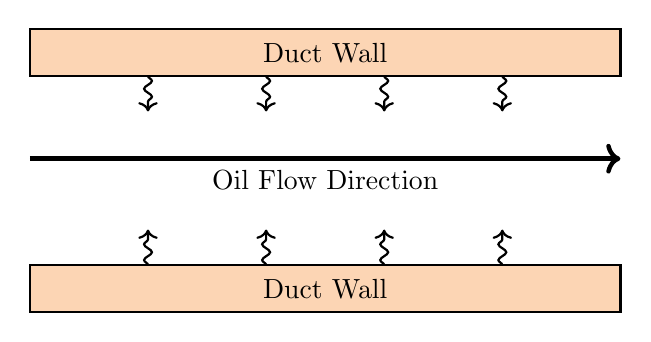
\begin{tikzpicture}[scale=1.5]
    % Define the thickness of the duct walls
    \newcommand{\ductthickness}{0.4}
    
    % Upper duct wall
    \fill[orangecolor] (0,1) rectangle ++(5,\ductthickness);
    \draw[thick] (0,1) rectangle ++(5,\ductthickness);
    
    % Lower duct wall
    \fill[orangecolor] (0,-1) rectangle ++(5,\ductthickness);
    \draw[thick] (0,-1) rectangle ++(5,\ductthickness);
    
    % Heat transfer arrows
    \foreach \x in {1,2,...,4}
        \draw[->, thick, decorate, decoration={snake, amplitude=0.5mm, segment length=2mm, post length=0.5mm}] (\x,0.8+\ductthickness/2) -- ++(0,-0.3);

    \foreach \x in {1,2,...,4}
        \draw[->, thick, decorate, decoration={snake, amplitude=0.5mm, segment length=2mm, post length=0.5mm}] (\x,-0.8+\ductthickness/2) -- ++(0,0.3);
    % Oil flow direction arrow
    \draw[->,fill=black,ultra thick] (0,0.3) -- ++(5,0) node[midway,below] {Oil Flow Direction};

    % Labels for the duct walls
    \node at (2.5,1+\ductthickness/2) {Duct Wall};
    \node at (2.5,-1+\ductthickness/2) {Duct Wall};
\end{tikzpicture}
\end{document}
